\documentclass[12pt]{article}
\usepackage[margin=2.5cm]{geometry}
\usepackage{enumerate}
\usepackage{amsfonts}
\usepackage{amsmath}
\usepackage{fancyhdr}
\usepackage{amsmath}
\usepackage{amssymb}
\usepackage{amsthm}
\usepackage{mdframed}
\usepackage{graphicx}
\usepackage{subcaption}
\usepackage{adjustbox}
\usepackage{listings}
\usepackage{xcolor}
\usepackage{soul}
\usepackage{booktabs}
\usepackage[utf]{kotex}
\usepackage{hyperref}

\definecolor{codegreen}{rgb}{0,0.6,0}
\definecolor{codegray}{rgb}{0.5,0.5,0.5}
\definecolor{codepurple}{rgb}{0.58,0,0.82}
\definecolor{backcolour}{rgb}{0.95,0.95,0.92}

\lstdefinestyle{mystyle}{
    backgroundcolor=\color{backcolour},
    commentstyle=\color{codegreen},
    keywordstyle=\color{magenta},
    numberstyle=\tiny\color{codegray},
    stringstyle=\color{codepurple},
    basicstyle=\ttfamily\footnotesize,
    breakatwhitespace=false,
    breaklines=true,
    captionpos=b,
    keepspaces=true,
    numbers=left,
    numbersep=5pt,
    showspaces=false,
    showstringspaces=false,
    showtabs=false,
    tabsize=1
}

\lstset{style=mystyle}

\pagestyle{fancy}
\renewcommand{\headrulewidth}{0.4pt}
\lhead{CSC 373}
\rhead{Worksheet 5 Solution}

\begin{document}
\title{CSC373 Worksheet 5 Solution}
\maketitle

\bigskip

\begin{enumerate}[1.]
    \item

    \bigskip

    \begin{proof}

    Assume that a flow network $G = (V,E)$ violates the assumption that the
    network contains a path $s \rightsquigarrow v \rightsquigarrow t$ for all
    vertices $v \in V$. Let $u$ be a vertex for which there is no path $s \rightsquigarrow u \rightsquigarrow t$.

    \bigskip

    I must show such that there is no flow at vertex $u$. That is, there exists a
    maximum flow $f$ in $G$ such that $f(u,v) = f(v,u) = 0$ for all vertices $v \in V$.

    \bigskip

    Assume for the sake of contradiction that there is some vertex $u$ with flow $f$.
    That is, there exists some vertices $v \in V$ such that $f(u,v) > 0$ or $f(v,u) > 0$.

    \bigskip

    I see that three cases follows, and I will prove each separately.

    \bigskip

    \begin{enumerate}[1.]
        \item \textbf{Cases 1:} $f(u,v) = 0$ and $f(v,u) > 0$

        \bigskip

        Here, assume that $f(u,v) = 0$ for all $v \in V$ and $f(v,u) > 0$ for some $v \in V$.

        \bigskip

        Then, we can write $\sum\limits_{v \in V} f(u,v) = 0$ and $\sum\limits_{v \in V} f(v,u) > 0$

        \bigskip

        But this violates the flow conservation property (i.e $\sum\limits_{v \in V} f(u,v) = \sum\limits_{v \in V} f(v,u)$)

        \bigskip

        Thus, by proof by contradiction, $f(u,v) = 0$ and $f(v,u) = 0$ for all $v \in V$ and
        all $u \in V$ with no path $s \rightsquigarrow u \rightsquigarrow t$.

        \bigskip

        \item \textbf{Cases 2:} $f(u,v) > 0$ and $f(v,u) = 0$

        \bigskip

        Here, assume that $f(u,v) > 0$ for some $v \in V$ and $f(v,u) = 0$ for all $v \in V$.

        \bigskip

        Then, by similar work as case 1, the same result follows.

        \bigskip

        \item \textbf{Cases 3:} $f(u,v) > 0$ and $f(v,u) > 0$

        \bigskip

        Here, assume that $f(u,v) > 0$ and $f(v,u) > 0$ for some $v \in V$.

        \bigskip

        Since $s \rightsquigarrow v \rightsquigarrow t$ and $u$ is connected by some vertices $v$,
        we can write $s \rightsquigarrow u \rightsquigarrow t$.

        \bigskip

        Then, this violates the fact in header that the vertex $u$ has no path $s \rightsquigarrow u \rightsquigarrow t$.

        \bigskip

        Thus, by proof by contradiction, $f(u,v) = 0$ and $f(v,u) = 0$ for all $v \in V$ and
        all $u \in V$ with no path $s \rightsquigarrow u \rightsquigarrow t$.

    \end{enumerate}

    \end{proof}

    \bigskip

    % \underline{\textbf{Rough Works:}}

    % \bigskip

    % Assume that a flow network $G = (V,E)$ violates the assumption that the
    % network contains a path $s \rightsquigarrow v \rightsquigarrow t$ for all
    % vertices $v \in V$. Let $u$ be a vertex for which there is no path $s \rightsquigarrow u \rightsquigarrow t$.

    % \bigskip

    % I must show such that there is no flow at vertex $u$. That is, there exists a
    % maximum flow $f$ in $G$ such that $f(u,v) = f(v,u) = 0$ for all vertices $v \in V$.

    % \bigskip

    % Assume for the sake of contradiction that there is some vertex $u$ with flow $f$.
    % That is, there exists some vertices $v \in V$ such that $f(u,v) > 0$ or $f(v,u) > 0$.

    % \bigskip

    % I see that three cases follows, and I will prove each separately.

    % \bigskip

    % \begin{enumerate}[1.]
    %     \item \textbf{Cases 1:} $f(u,v) = 0$ and $f(v,u) > 0$

    %     \bigskip

    %     Here, assume that $f(u,v) = 0$ for all $v \in V$ and $f(v,u) > 0$ for some $v \in V$.

    %     \bigskip

    %     \begin{itemize}
    %         \item Show that $\sum\limits_{v \in V} f(u,v) = 0$ and $\sum\limits_{v \in V} f(v,u) > 0$

    %         \begin{mdframed}
    %         Then, we can write $\sum\limits_{v \in V} f(u,v) = 0$ and $\sum\limits_{v \in V} f(v,u) > 0$
    %         \end{mdframed}

    %         \item Show that this violates flow conservation [contradiction]

    %         \begin{mdframed}
    %         But this violates the flow conservation property (i.e $\sum\limits_{v \in V} f(u,v) = \sum\limits_{v \in V} f(v,u)$)
    %         \end{mdframed}

    %         \item Conclude that $f(u,v) = 0$ and $f(v,u) = 0$

    %         \begin{mdframed}
    %         Thus, by proof by contradiction, $f(u,v) = 0$ and $f(v,u) = 0$ for all $v \in V$ and
    %         all $u \in V$ with no path $s \rightsquigarrow u \rightsquigarrow t$.
    %         \end{mdframed}
    %     \end{itemize}

    %     \begin{mdframed}
    %     Here, assume that $f(u,v) = 0$ for all $v \in V$ and $f(v,u) > 0$ for some $v \in V$.

    %     \bigskip

    %     Then, we can write $\sum\limits_{v \in V} f(u,v) = 0$ and $\sum\limits_{v \in V} f(v,u) > 0$

    %     \bigskip

    %     But this violates the flow conservation property (i.e $\sum\limits_{v \in V} f(u,v) = \sum\limits_{v \in V} f(v,u)$)

    %     \bigskip

    %     Thus, by proof by contradiction, $f(u,v) = 0$ and $f(v,u) = 0$ for all $v \in V$ and
    %     all $u \in V$ with no path $s \rightsquigarrow u \rightsquigarrow t$.
    %     \end{mdframed}

    %     \item \textbf{Cases 2:} $f(u,v) > 0$ and $f(v,u) = 0$

    %     \begin{mdframed}
    %     By similar work as case 1, the same result follows.
    %     \end{mdframed}

    %     \item \textbf{Cases 3:} $f(u,v) > 0$ and $f(v,u) > 0$

    %     \bigskip

    %     Here, assume that $f(u,v) > 0$ and $f(v,u) > 0$ for some $v \in V$.

    %     \bigskip

    %     \begin{itemize}
    %         \item Write that the path $s \rightsquigarrow u \rightsquigarrow t$ exists

    %         \begin{mdframed}
    %         Since $s \rightsquigarrow v \rightsquigarrow t$ and $u$ is connected by some vertices $v$,
    %         we can write $s \rightsquigarrow u \rightsquigarrow t$.
    %         \end{mdframed}

    %         \item Write that this results in contradiction to the header that
    %         a vertex $u$ has no path $s \rightsquigarrow u \rightsquigarrow t$.

    %         \begin{mdframed}
    %         Then, this violates the fact in header that the vertex $u$ has no path $s \rightsquigarrow u \rightsquigarrow t$.
    %         \end{mdframed}

    %         \item Conclude that $f(u,v) = 0$ and $f(v,u) = 0$

    %         \begin{mdframed}
    %             Thus, by proof by contradiction, $f(u,v) = 0$ and $f(v,u) = 0$ for all $v \in V$ and
    %             all $u \in V$ with no path $s \rightsquigarrow u \rightsquigarrow t$.
    %         \end{mdframed}
    %     \end{itemize}

    %     \begin{mdframed}

    %     Here, assume that $f(u,v) > 0$ and $f(v,u) > 0$ for some $v \in V$.

    %     \bigskip

    %     Since $s \rightsquigarrow v \rightsquigarrow t$ and $u$ is connected by some vertices $v$,
    %     we can write $s \rightsquigarrow u \rightsquigarrow t$.

    %     \bigskip

    %     Then, this violates the fact in header that the vertex $u$ has no path $s \rightsquigarrow u \rightsquigarrow t$.

    %     \bigskip

    %     Thus, by proof by contradiction, $f(u,v) = 0$ and $f(v,u) = 0$ for all $v \in V$ and
    %         all $u \in V$ with no path $s \rightsquigarrow u \rightsquigarrow t$.

    %     \end{mdframed}
    % \end{enumerate}

    \bigskip

    \underline{\textbf{Notes}}

    \begin{itemize}
        \item \textbf{Maximum Flow:}

        \begin{itemize}
            \item Finds a flow of maximum value $^{[1]}$

            \bigskip

            \underline{\textbf{Example}}

            \bigskip

            \begin{center}
            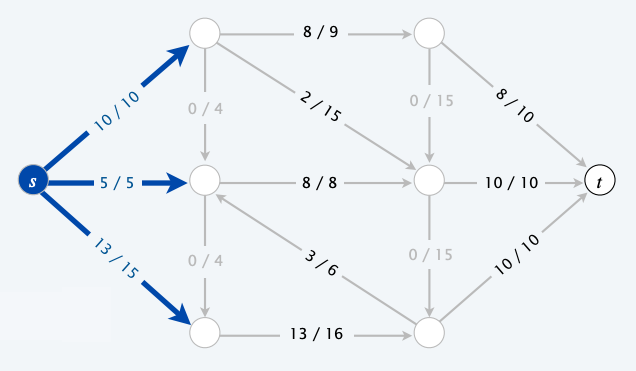
\includegraphics[width=0.7\linewidth]{images/worksheet_5_solution_3.png}
            \end{center}

            \bigskip

            Here, the maximum flow is $10 + 5 + 13 = 28$
        \end{itemize}

        \bigskip

        \item \textbf{Flow Network:}
        \begin{itemize}
            \item $G = (V,E)$ is a directed graph in which each edge $(u,v) \in E$
            has a nonnegative capacity $c(u,v) \geq 0$.
            \item Two vertices must exist: \textbf{source} s and \textbf{sink} t
            \item \textbf{path} from source $s$ to vertax $v$ to sink $t$ is represented by $s \rightsquigarrow v \rightsquigarrow t$

        \end{itemize}

        \bigskip

        \begin{center}
        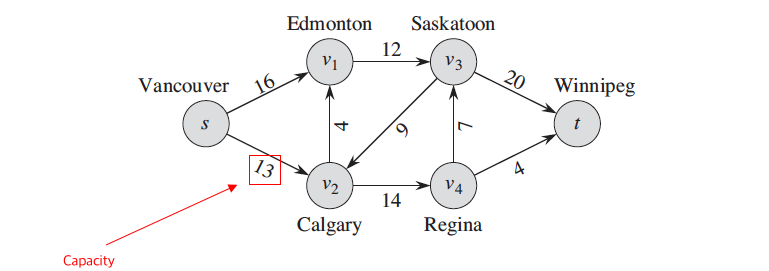
\includegraphics[width=0.9\linewidth]{images/worksheet_5_solution_1.png}
        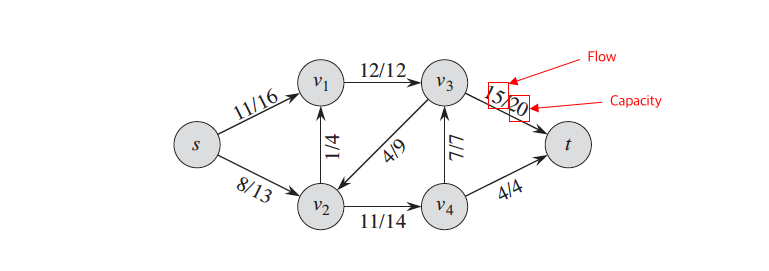
\includegraphics[width=0.9\linewidth]{images/worksheet_5_solution_2.png}
        \end{center}

        \item \textbf{Capacity:}

        \begin{itemize}
            \item Is a non-negative function $f: V \times V \to \mathbb{R}_{\geq 0}$
            \item Has \textbf{capacity constraint} where for all $u,v \in V$ $0 \leq f(u,v) \leq c(u,v)$

            \begin{itemize}
                \item Means flow cannot be above capacity constraint
            \end{itemize}
        \end{itemize}

        \item \textbf{Flow:}

        \begin{itemize}
            \item Is a real valued function $f: V \times V \to \mathbb{R}$ in $G$
            \item Satisfies \textbf{capacity constraint} (i.e for all $u,v \in V$, $0 \leq f(u,v) \leq c(u,v)$)
            \item Satisfies \textbf{flow conservation}

            \bigskip

            For all $u \in V - \{s,t\}$, we require

            \bigskip

            \begin{align}
            \sum\limits_{v \in V} f(v,u) = \sum\limits_{v \in V} f(u,v)
            \end{align}

            \bigskip

            \begin{itemize}
                \item Means flow into vertex $u$ is the same as flow going out of vertex $u$. $^{[1]}$
                \item $\sum\limits_{v \in V} f(u,v)$ means flow \underline{out of} vertex $u$
                \item $\sum\limits_{v \in V} f(v,u)$ means flow \underline{into} vertex $u$
                \item $v \in V$ in $\sum\limits_{v \in V} f(u,v)$ means all vertices that are an edge away from vertex $u$
            \end{itemize}

            \bigskip

            \underline{\textbf{Example:}}

            \begin{center}
            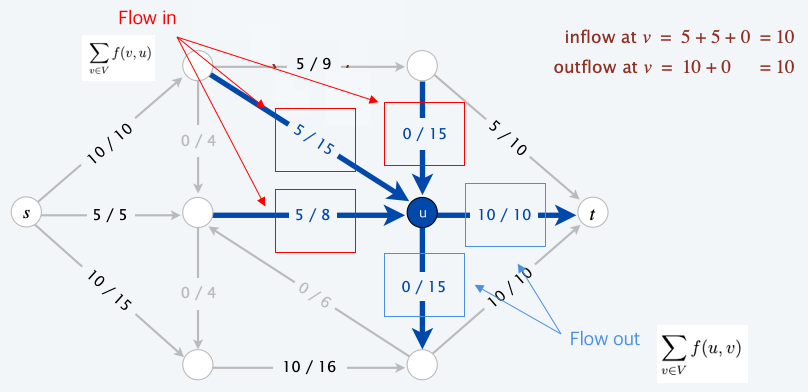
\includegraphics[width=0.9\linewidth]{images/worksheet_5_solution_4.png}
            \end{center}


        \end{itemize}
    \end{itemize}

    \bigskip

    \underline{\textbf{References}}

    \bigskip

    \begin{enumerate}[1)]
        \item Princeton University, Network Flow 1, \href{https://www.cs.princeton.edu/~wayne/kleinberg-tardos/pdf/07NetworkFlowI.pdf}{link}
    \end{enumerate}

    \item

    \bigskip

    I need to formulate the problem of determining whether both of professor Adam's two children can go to the same school
    as maximum-flow problem.

    \bigskip

    The problem statement tells us the following:

    \bigskip

    \begin{enumerate}[1.]
        \item There is 1 supersource (location of home)
        \item There is 1 sink (location of school)
        \item There are two sources ($s_1$ as child 1, $s_2$ as child 2)
        \item Edge $(u,v)$ has capacity of 0 or more (0 representing unavailable sidewalk, 1 for sidewalk with capacity of 1, 2 for street with capacity of 2 and so on)
        \item Each vertex represents corner of intersection, and two children can have their paths crossing here.
        \item Has flow of 2, 1 or 0 (1 is where one of the two children walking on the road. 0 is none.)
    \end{enumerate}

    \bigskip

    Here we are to find whether children must go on to a vertex and out to the same edge with the flow of 2,
    or determine whether there is only edge to school with capacity of 1 or less.

    \bigskip

    If none, then both children can safely go to school.

    \bigskip

    \begin{center}
    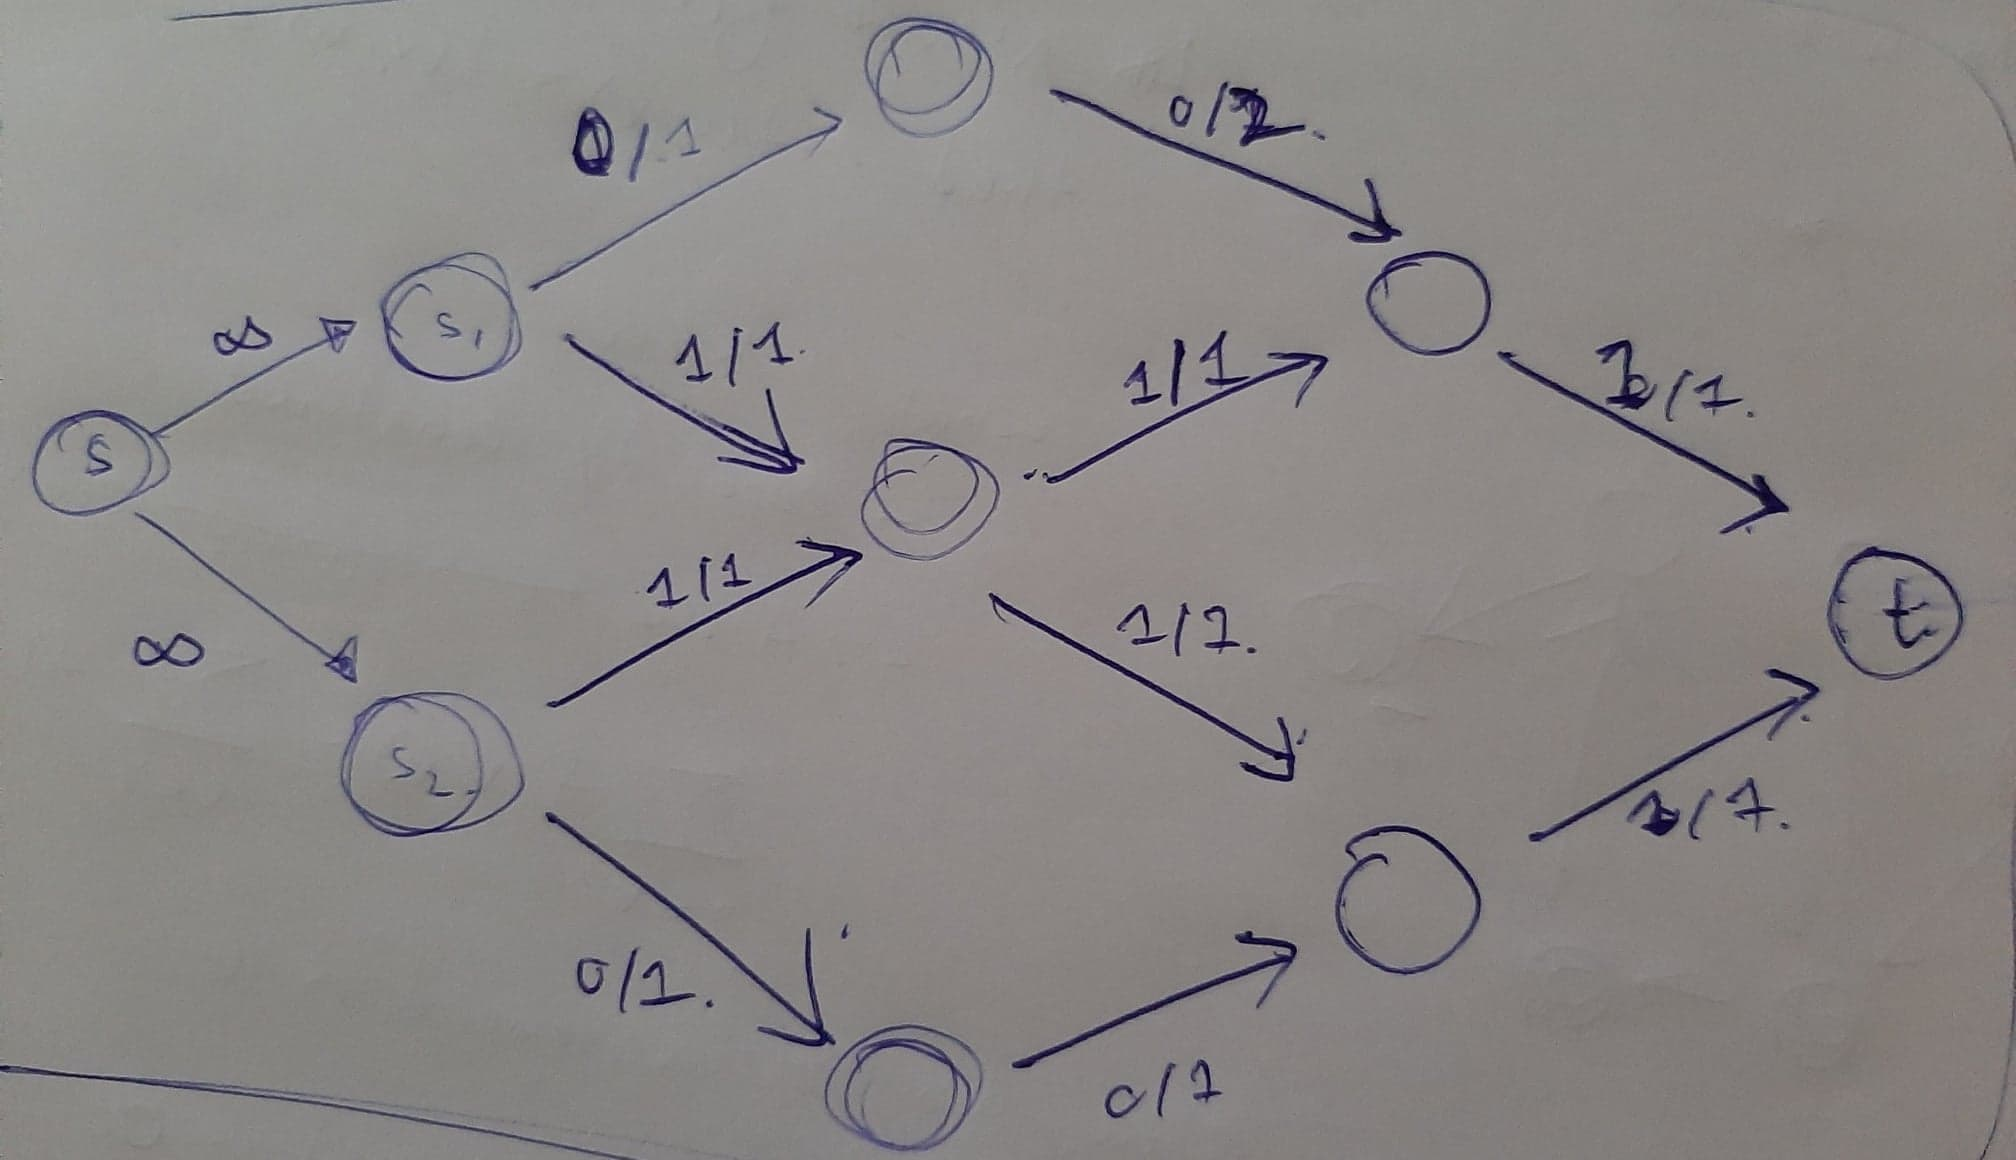
\includegraphics[width=0.7\linewidth]{images/worksheet_5_solution_7.jpg}
    \end{center}

    \bigskip

    % \underline{\textbf{Rough Works:}}

    % \bigskip

    % I need to formulate the problem of determining whether both of professor Adam's two children can go to the same school
    % as maximum-flow problem.

    % \bigskip

    % The problem statement tells us the following:

    % \bigskip

    % \begin{enumerate}[1.]
    %     \item There is 1 supersource (location of home)
    %     \item There is 1 sink (location of school)
    %     \item There are two sources ($s_1$ as child 1, $s_2$ as child 2)
    %     \item Edge $(u,v)$ has capacity of 0 or more (0 representing unavailable sidewalk, 1 for sidewalk with capacity of 1, 2 for street with capacity of 2 and so on)
    %     \item Each vertex represents corner of intersection, and two children can have their paths crossing here.
    %     \begin{itemize}
    %         \item But total inflow must equal total outflow (by flow conservation)
    %     \end{itemize}
    %     \item Has flow of 2, 1 or 0 (1 is where one of the two children walking on the road. 0 is none.)
    % \end{enumerate}

    % \bigskip

    % Here we are to find whether children must go on to a vertex and out to the same edge with the flow of 2,
    % or determine whether there is only edge to school with capacity of 1 or less.

    % \bigskip

    % If none, then both children can safely go to school.

    % \bigskip

    \underline{\textbf{Notes:}}

    \bigskip

    \begin{itemize}
        \item \textbf{Cross at a Corner}

        \begin{itemize}
            \item Means to walk across the street at a corner of the intersection.

            \bigskip

            \begin{center}
            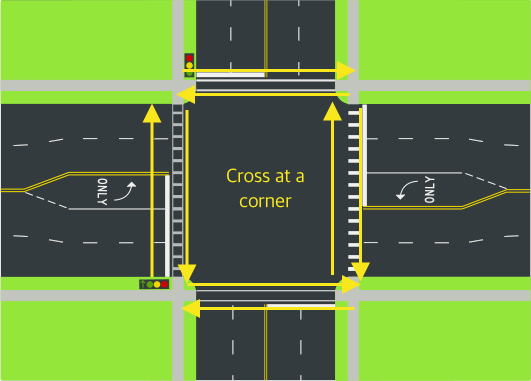
\includegraphics[width=0.7\linewidth]{images/worksheet_5_solution_5.png}
            \end{center}
        \end{itemize}

        \item \textbf{Multiple Sources and Sinks}

        \begin{itemize}
            \item Has edges $(s, s_i)$ where $i = 1 ... n$ and $(t_j, t)$ where $j = 1 ... n$
            with capacity of $\infty$
        \end{itemize}

        \bigskip

        \underline{\textbf{Example:}}

        \bigskip

        Lucky Puck Company having a set of $m$ factories $\{s_1, s_2, ..., s_m\}$, and
        a set of $n$ warehourses and $n$ warehouses $\{t_1, t_2, ..., t_n\}$

        \bigskip

        \begin{center}
        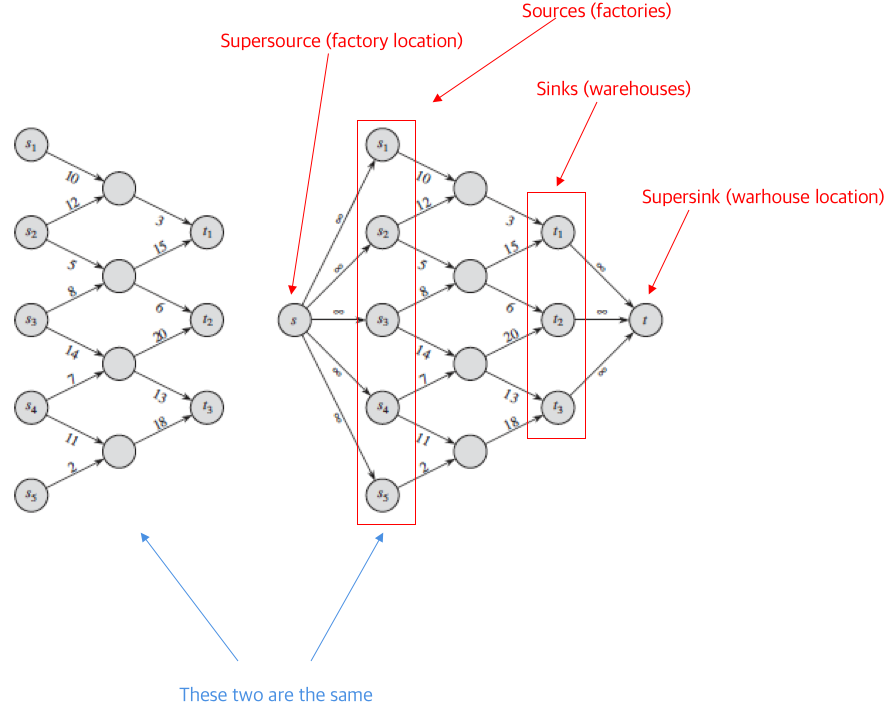
\includegraphics[width=0.9\linewidth]{images/worksheet_5_solution_6.png}
        \end{center}

    \end{itemize}

    \item

    \bigskip

    I need to show how to transform a flow network $G = (V,E)$ with vertex capacities
    into an equivalent flow network $G' = (V',E')$ without vertex capacities.

    \bigskip

    For each vertex capacities, change as follows.

    \begin{center}
    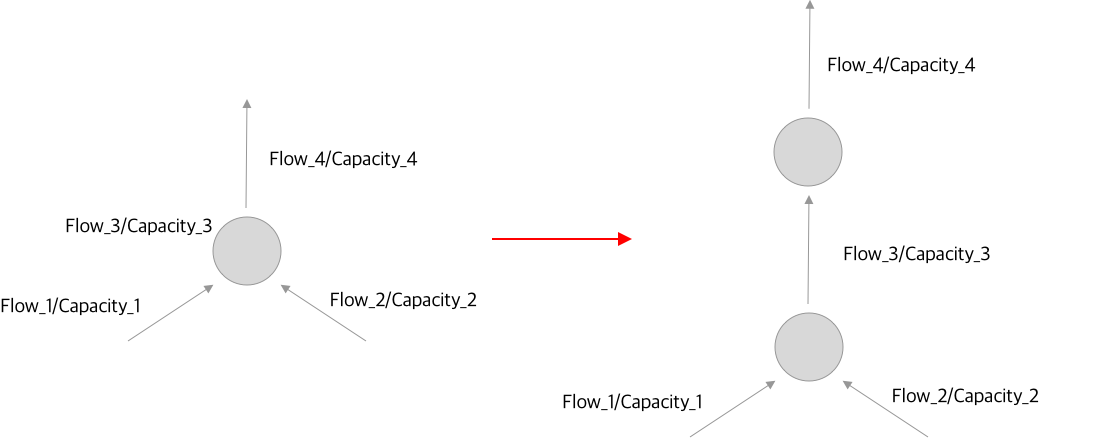
\includegraphics[width=0.9\linewidth]{images/worksheet_5_solution_8.png}
    \end{center}

    \bigskip

    After transformation, there will be $m$ more edges and verticies, where $m$
    represents the number of vertex capacities in $G$.

    \bigskip

    \underline{\textbf{Notes:}}

    \bigskip

    \begin{itemize}
        \item \textbf{Vertex Capacities}
        \begin{itemize}
            \item Each vertex $v$ has limit $l(v)$ on how much flow can pass through $v$
        \end{itemize}
    \end{itemize}

    \item

    \bigskip

    I need to show how to convert the problem of finding a flow $f$ that obeys the
    constraints into the problem of finding a maximum flow in a single
    source, single-sink flow network

    \bigskip

    The steps are as follows:

    \bigskip

    \begin{itemize}
        \item Combine all sources $s_i$ into a single source $s$
        \item Combine all sinks $t_j$ into a single sink $t$
        \item Connect source $s$ to each adjacent vertex $v$ with edge weight $\sum\limits_{i} f(s_i, v) = p_i$

        \begin{itemize}
            \item The total edge weight from $s$ should be $\sum\limits_{i} p_i$
        \end{itemize}

        \item Connect each adjacent vertex $v$ of t to $t$ with edge weight $\sum\limits_{j} f(v,t_j) = q_j$

        \begin{itemize}
            \item The total edge weight to $t$ should be $\sum\limits_{j} q_j$
        \end{itemize}


        \item Find a simple path from $s$ to $t$ with the maximum amount of total flow
    \end{itemize}

    \begin{center}
    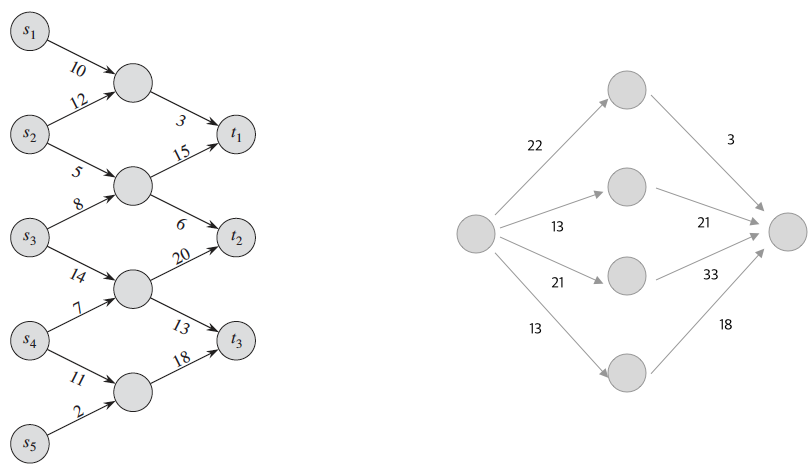
\includegraphics[width=0.9\linewidth]{images/worksheet_5_solution_16.png}
    \end{center}

    \bigskip

    \begin{mdframed}
        \underline{\textbf{Correct Solution:}}


        I need to show how to convert the problem of finding a flow $f$ that obeys the
        constraints into the problem of finding a maximum flow in a single
        source, single-sink flow network

        \bigskip

        The steps are as follows:

        \bigskip

        \begin{itemize}
            \item Combine all sources $s_i$ into a single source $s$
            \item Combine all sinks $t_j$ into a single sink $t$
            \item Connect source $s$ to each adjacent vertex $v$ with edge weight $\sum\limits_{i} f(s_i, v) = p_i$

            \begin{itemize}
                \item The total edge weight from $s$ should be $\sum\limits_{i} p_i$
            \end{itemize}

            \item Connect each adjacent vertex $v$ of t to $t$ with edge weight $\sum\limits_{j} f(v,t_j) = q_j$

            \begin{itemize}
                \item The total edge weight to $t$ should be $\sum\limits_{j} q_j$
            \end{itemize}


            \item Find a simple path from $s$ to $t$ with the maximum amount of total flow
        \end{itemize}

        \color{red}\underline{\textbf{Example}}\color{black}

        \begin{center}
        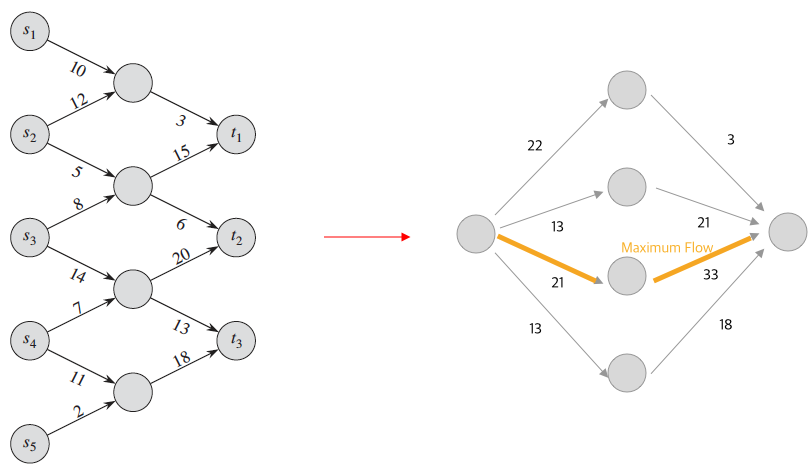
\includegraphics[width=0.9\linewidth]{images/worksheet_5_solution_17.png}
        \end{center}

    \end{mdframed}

    \bigskip

    % \underline{\textbf{Rough Works:}}

    % \bigskip

    % I need to show how to convert the problem of finding a flow $f$ that obeys the
    % constraints into the problem of finding a maximum flow in a single
    % source, single-sink flow network

    % \bigskip

    % The steps are as follows:

    % \bigskip

    % \begin{itemize}
    %     \item Combine all sources $s_i$ into a single source $s$
    %     \item Combine all sinks $t_j$ into a single sink $t$
    %     \item Connect source $s$ to each adjacent vertex $v$ with edge weight $\sum\limits_{i} f(s_i, v) = p_i$

    %     \begin{itemize}
    %         \item The total edge weight from $s$ should be $\sum\limits_{i} p_i$
    %     \end{itemize}

    %     \item Connect each adjacent vertex $v$ of t to $t$ with edge weight $\sum\limits_{j} f(v,t_j) = q_j$

    %     \begin{itemize}
    %         \item The total edge weight to $t$ should be $\sum\limits_{j} q_j$
    %     \end{itemize}


    %     \item Find a simple path from $s$ to $t$ with the maximum amount of total flow
    % \end{itemize}

    % \begin{center}
    % 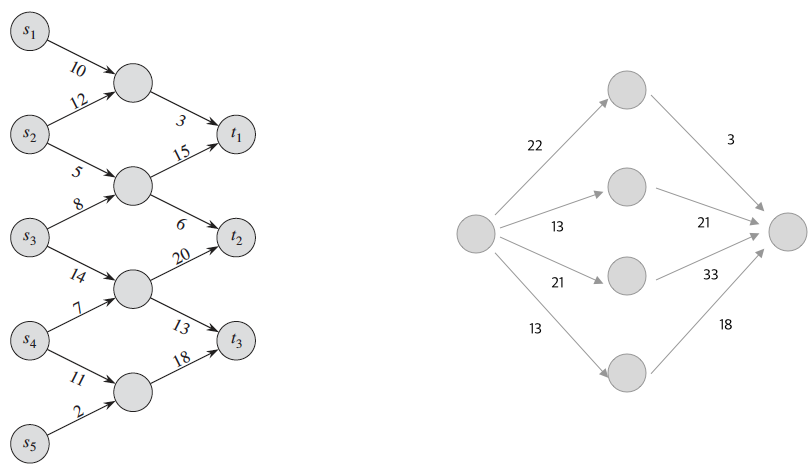
\includegraphics[width=0.9\linewidth]{images/worksheet_5_solution_16.png}
    % \end{center}


    % \bigskip

    \underline{\textbf{Notes:}}

    \bigskip

    \begin{itemize}
        \item \textbf{Ford-Fulkerson Method}

        \begin{itemize}
            \item Is a greedy algorithm that solves the maximum-flow problem
            \begin{itemize}
                \item Determines maximum flow from start vertex to sink vertex in a graph
            \end{itemize}
            \item Called method (not algorithm) because several different implementations
            with different running time is used
        \end{itemize}

        \begin{center}
        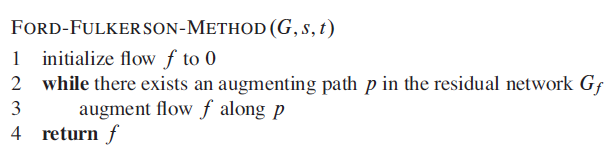
\includegraphics[width=0.9\linewidth]{images/worksheet_5_solution_9.png}
        \end{center}

        \item \textbf{Residual Network}
        \begin{itemize}
            \item Indicates how muh more flow is allowed in each edge in the network graph $^{[1]}$
            \item Consists of edges with capacities that represents how we can change the flow on edges of $G$.
            \item Provides roadmap for adding flow to the original flow network
        \end{itemize}

        \bigskip

        \begin{center}
        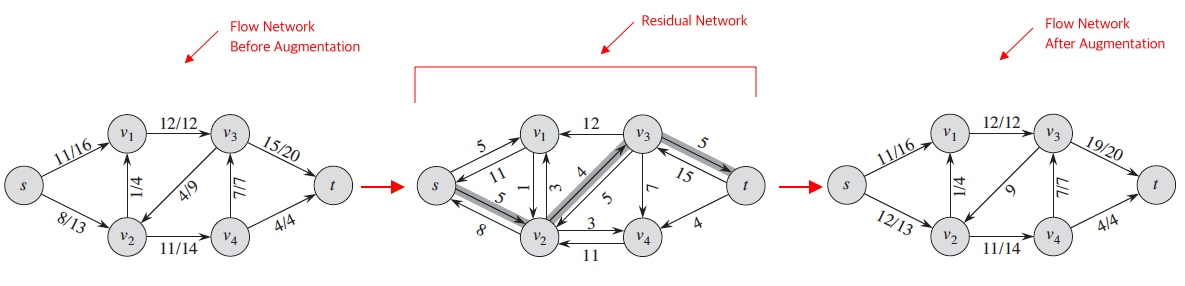
\includegraphics[width=\linewidth]{images/worksheet_5_solution_12.png}
        \end{center}

        \bigskip

        \underline{\textbf{Steps}}

        \bigskip

        \begin{enumerate}[1)]
            \item \textbf{$Flow = Capacity$:} Opposite arrow

            \begin{center}
            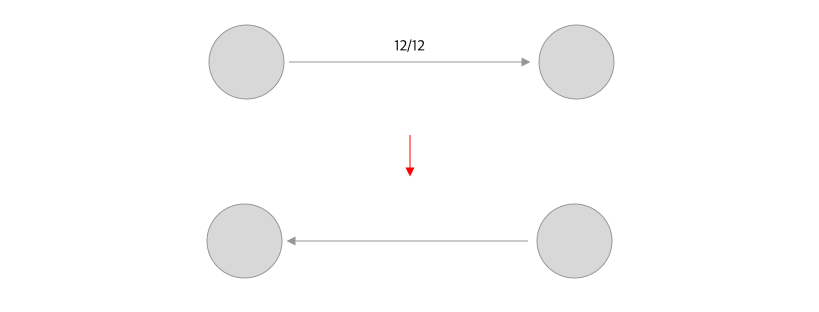
\includegraphics[width=0.8\linewidth]{images/worksheet_5_solution_10.png}
            \end{center}

            \item \textbf{$Flow < Capacity$:}

            \begin{itemize}
                \item \textbf{$Flow$:} Oppisite Arrow
                \item \textbf{$Capacity - Flow$:} Current Arrow
            \end{itemize}

            \begin{center}
            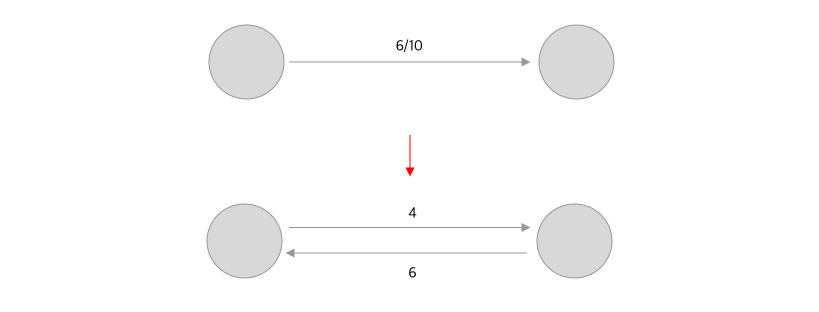
\includegraphics[width=0.8\linewidth]{images/worksheet_5_solution_11.png}
            \end{center}
        \end{enumerate}

        \bigskip

        \item \textbf{Augmenting Path}

        \begin{itemize}
            \item Is a path from source S to sink T where you can increase the amount of flow
            \item Is a path that doesn't contain cycle (simple path) $^{[2]}$

            \begin{center}
            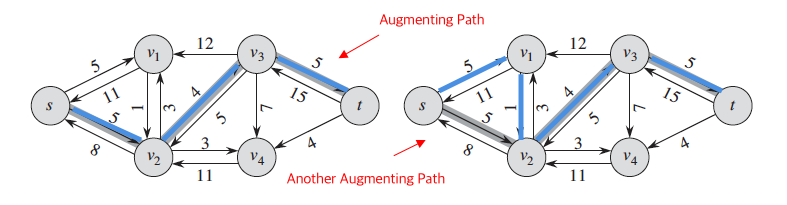
\includegraphics[width=\linewidth]{images/worksheet_5_solution_13.png}
            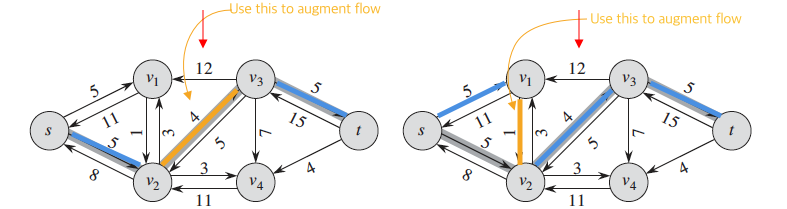
\includegraphics[width=\linewidth]{images/worksheet_5_solution_14.png}
            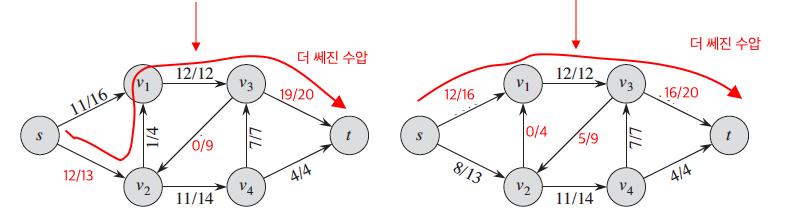
\includegraphics[width=\linewidth]{images/worksheet_5_solution_15.png}
            \end{center}

            \item Edge $(u,v)$ of an augmented path can be increased
            by upto $c_f(u,v)$ withhout violating the capacity constraint
        \end{itemize}

        \item \textbf{Augmentation}

        \begin{itemize}
            \item 한국어로 '불필요한 수압 decrease 해서 앞으로 가는 수압 더 쎄게 만들기'
            \item Is symbolized by $f \uparrow f'$

            \begin{itemize}
                \item $f$ is a flow in $G$
                \item $f'$ is a flow in the residual network $G_f$
            \end{itemize}
        \end{itemize}

    \end{itemize}

    \bigskip

    \underline{\textbf{References}}

    \bigskip

    \begin{enumerate}[1)]
        \item Hacker Earth, Maximum Flow, \href{https://www.hackerearth.com/practice/algorithms/graphs/maximum-flow/tutorial/}{link}
        \item Stack Overflow, What Exactly Is Augmentation Path, \href{https://stackoverflow.com/questions/10397118/what-exactly-is-augmenting-path}{link}
    \end{enumerate}

    \item
    \setcounter{equation}{0}
    \bigskip

    The augmented flow satisfies flow conservation, but not capacity constraint.

    \bigskip

    \begin{proof}
    Let $G = (V,E)$ be a flow network with sources $s$ and sink $t$. Let $f,f'$
    be a flow in $G$. Let $(u,v)$ be an edge in $E$ where $u \in V - \{s,t\}$ and
    $v \in V$. We note that if $(u,v) \in E$, then $(v,u) \notin E$ and $f(v,u) = 0$. Thus,
    we can re-write the definition of flow augmentation (equation (26.4)) as

    \begin{align}
        (f \uparrow f')(u,v) &= \begin{cases}
            f(u,v) + f'(u,v) & [\text{If $(u,v) \in E$}]\\
            0 & [\text{Otherwise}]
        \end{cases}
    \end{align}

    which implies that the value of the augmentation of flow $f \uparrow f'$
    on edge $(u,v)$ is the sum of flow $f(u,v)$ and $f'(u,v)$ in $G$.

    \bigskip

    I need to show if the augmented flow of $f$ and $f'$ $\in G$ and satisfy the
    flow conservation property but not capacity constraint.

    \bigskip

    I will do so in parts

    \begin{itemize}
        \item \textbf{Part 1: Proving that $f \uparrow f'$ satisfies the flow conservation property}

        \bigskip

        Here I prove that the augmented flow satisfies flow conservation. That is,

        \begin{align}
        \sum\limits_{v \in V} f \uparrow f' (u,v) = \sum\limits_{v \in V} f \uparrow f' (v,u)
        \end{align}.

        \bigskip

        And indeed we have,

        \begin{align}
            \sum\limits_{v \in V} f \uparrow f' (u,v) &= \sum\limits_{v \in V} f(u,v) + f'(u,v) & [\text{By augmentation def.}]\\
            &= \sum\limits_{v \in V} f(u,v) + \sum\limits_{v \in V} f'(u,v)\\
            &= \sum\limits_{v \in V} f(v,u) + \sum\limits_{v \in V} f'(v,u) & [\text{By flow conserv. of $f$ and $f'$}]\\
            &= \sum\limits_{v \in V} f(v,u) + f'(v,u)\\
            &= f \uparrow f' (v,u)
        \end{align}

        \bigskip

        \item \textbf{Part 2: Disproving that $f \uparrow f'$ satisfies the capacity constraint}

        \bigskip

        Here, I need to disprove that the augmented flow satisfies capacity constraint. That is,

        \begin{align}
            (f \uparrow f')(u,v) > c(u,v)
        \end{align}

        \bigskip

        Let $f(u,v) = f'(u,v) = 10$ and $c(u,v) = 8$.

        \bigskip

        Then, we can write $(f \uparrow f')(s,t) = 20$ and $c(u,v) = 8$.

        \bigskip

        Thus, we can conclude the augmentation of flow doesn't satisfy capacity constraint.
    \end{itemize}

    \end{proof}

    % \underline{\textbf{Rough Works:}}

    % \bigskip


    % \bigskip

    % I need to show if the augmented flow of $f$ and $f'$ $\in G$ and satisfy the
    % flow conservation property but not capacity constraint.

    % \bigskip

    % \begin{itemize}
    %     \item Proving that $f \uparrow f'$ satisfies the flow conservation property

    %     \bigskip

    %     \begin{mdframed}

    %     Let $G = (V,E)$ be a flow network with sources $s$ and sink $t$. Let $f,f'$
    %     be a flow in $G$. Let $(u,v)$ be an edge in $E$ where $u \in V - \{s,t\}$ and
    %     $v \in V$. We note that if $(u,v) \in E$, then $(v,u) \notin E$ and $f(v,u) = 0$. Thus,
    %     we can re-write the definition of flow augmentation (equation (26.4)) as

    %     \begin{align}
    %         (f \uparrow f')(u,v) &= \begin{cases}
    %             f(u,v) + f'(u,v) & [\text{If $(u,v) \in E$}]\\
    %             0 & [\text{Otherwise}]
    %         \end{cases}
    %     \end{align}

    %     which implies that the value of the augmentation of flow $f \uparrow f'$
    %     on edge $(u,v)$ is the sum of flow $f(u,v)$ and $f'(u,v)$ in $G$. We now prove
    %     that the augmented flow satisfies flow conservation. That is,

    %     \begin{align}
    %     \sum\limits_{v \in V} f \uparrow f' (u,v) = \sum\limits_{v \in V} f \uparrow f' (v,u)
    %     \end{align}.

    %     \bigskip

    %     And indeed we have,

    %     \begin{align}
    %         \sum\limits_{v \in V} f \uparrow f' (u,v) &= \sum\limits_{v \in V} f(u,v) + f'(u,v) & [\text{By augmentation def.}]\\
    %         &= \sum\limits_{v \in V} f(u,v) + \sum\limits_{v \in V} f'(u,v)\\
    %         &= \sum\limits_{v \in V} f(v,u) + \sum\limits_{v \in V} f'(v,u) & [\text{By flow conserv. of $f$ and $f'$}]\\
    %         &= \sum\limits_{v \in V} f(v,u) + f'(v,u)\\
    %         &= f \uparrow f' (v,u)
    %     \end{align}

    %     \end{mdframed}

    %     \bigskip

    %     \item Disproving that $f \uparrow f'$ satisfies the capacity constraint

    %     \bigskip

    %     \underline{\textbf{Predicate Logic:}} $\forall f,f' \in G$, $\forall (u,v) \in E \text{ where $u,v \in V$}$,
    %     $0 \leq (f \uparrow f')(u,v) \land (f \uparrow f')(u,v) \leq c(u,v)$

    %     \bigskip

    %     \underline{\textbf{Negation of Predicate Logic:}} $\exists f,f' \in G$, $\exists (u,v) \in E \text{ where $u,v \in V$}$,
    %     $0  > (f \uparrow f')(u,v) \land (f \uparrow f')(u,v) > c(u,v)$

    %     \begin{mdframed}
    %     Let $G = (V,E)$ be a flow network with sources $s$ and sink $t$. Let $f,f'$
    %     be a flow in $G$. Let $(u,v)$ be an edge in $E$ where $u \in V - \{s,t\}$ and
    %     $v \in V$. We note that if $(u,v) \in E$, then $(v,u) \notin E$ and $f(v,u) = 0$. Thus,
    %     we can re-write the definition of flow augmentation (equation (26.4)) as

    %     \begin{align}
    %         (f \uparrow f')(u,v) &= \begin{cases}
    %             f(u,v) + f'(u,v) & [\text{If $(u,v) \in E$}]\\
    %             0 & [\text{Otherwise}]
    %         \end{cases}
    %     \end{align}

    %     which implies that the value of the augmentation of flow $f \uparrow f'$
    %     on edge $(u,v)$ is the sum of flow $f(u,v)$ and $f'(u,v)$ in $G$. We now disprove
    %     that the augmented flow satisfies capacity constraint. That is,

    %     \begin{align}
    %         (f \uparrow f')(u,v) > c(u,v)
    %     \end{align}

    %     \bigskip

    %     Let $f(u,v) = f'(u,v) = 10$ and $c(u,v) = 8$.

    %     \bigskip

    %     Then, we can write $(f \uparrow f')(s,t) = 20$ and $c(u,v) = 8$.

    %     \bigskip

    %     Thus, we can conclude the augmentation of flow doesn't satisfy capacity constraint.
    %     \end{mdframed}
    % \end{itemize}

    \bigskip

    \underline{\textbf{Notes:}}

    \bigskip

    \begin{itemize}
        \item I need clarification from professor about the meaning of $f' \in G$.
        Is $f'$ a flow from flow network or residual network?
        \item I feel I am struggling because I am jumping to solution without understanding the problem
        \item I feel constructing a predicate logic would have helped to better understand this problem
        \item Noticed that a solution in University of Texas really elaborated on $f \uparrow f'(u,v)$
        before moving onto strategizing and constructing a solution

        \begin{center}
        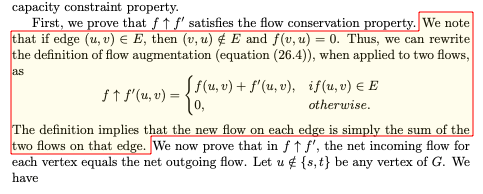
\includegraphics[width=0.8\linewidth]{images/worksheet_5_solution_18.png}
        \end{center}

        \item Noticed that a solution in University of Texas made quick sketches
        before laying the outline of proof

        \item \textbf{Flow Network (cont'd)} [Important!]

        \begin{itemize}
            \item Flow network requires that

            \begin{enumerate}[1)]
                \item $G = (V,E)$ is a directed graph
                \item each edge $(u,v) \in E$ has a non-negative capacity $c(u,v) \geq 0$
                \item \color{red}\ul{If $E$ contains an edge $(u,v)$, then there is no edge $(v,u)$ in the reverse direction (no anti-parallel edge)}\color{black}
            \end{enumerate}
        \end{itemize}

        \item \textbf{Augmentation (cont'd)}

        \begin{itemize}
            \item Flow value can be increased by

            \begin{align}
                c_f(p) = \min_{(u,v) \in p} c_f(u,v)
            \end{align}

            \bigskip

            \underline{\textbf{Example:}}

            \begin{center}
            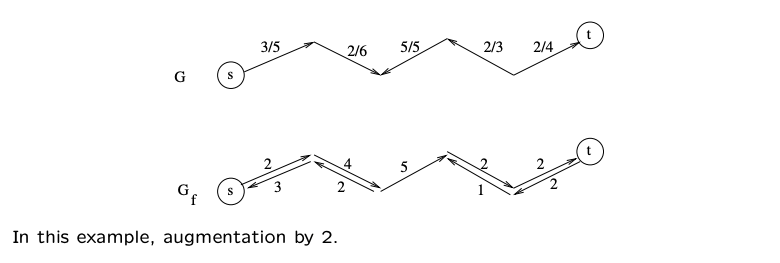
\includegraphics[width=\linewidth]{images/worksheet_5_solution_20.png}
            \end{center}


            \item Augmentation of flow $f$ by $f'$ or $f \uparrow f'$ is a function
            $V \times V \to \mathbb{R}$ is defined by


            \begin{align}
                (f \uparrow f')(u,v) &= \begin{cases}
                    f(u,v) + f'(u,v) - f'(v,u) & [\text{If $(u,v) \in E$}]\\
                    0 & [\text{Otherwise}]
                \end{cases}
            \end{align}

            \item \color{red}\ul{Augmentation of flow $f \uparrow f'$ is the sum of flow on edge $(u,v)$
            in both flow network $G$ and residual network $G'$}\color{black}

            \begin{center}
            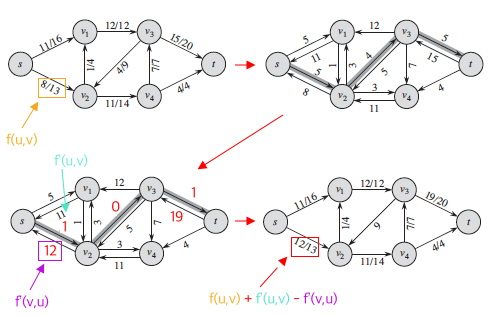
\includegraphics[width=0.8\linewidth]{images/worksheet_5_solution_19.png}
            \end{center}


            [\color{red}NOTE!!\color{black}] I really need to ask professor about this. I can't seem to
            understand using simple example why $f \uparrow f'(u,v) = f(u,v) + f'(u,v) - f'(v,u)$.
        \end{itemize}

        \item \textbf{Proof of flow conservation for $f \uparrow f'$ when $f \in G$ and $f' \in G_f$}
        \setcounter{equation}{0}
        \bigskip

        Let $G = (V,E)$ be a flow network with sources $s$ and sink $t$. Let $f$
        be a flow in $G$. Let $G_f$ be a residual network of $G$ induced by $f$ and let $f'$ be
        a flow in $G_f$. Let $(u,v)$ be an edge in $E$ where $u \in V - \{s,t\}$ and $v \in V$. We note that if $(u,v) \in E$, then $(v,u) \notin E$ and $f(v,u) = 0$. Thus,
        the definition


        \begin{align}
            (f \uparrow f')(u,v) &= \begin{cases}
                f(u,v) + f'(u,v) - f'(v,u) & [\text{If $(u,v) \in E$}]\\
                0 & [\text{Otherwise}]
            \end{cases}
        \end{align}

        \bigskip

        implies that the augmented flow $f \uparrow f'(u,v)$ on edge $(u,v)$ is the
        sum of flow $f(u,v)$ in flow network $G$ and flow $f'(u,v)$ minus its antiparallel
        flow $-f'(v,u)$ in residual flow network $G'$.

        \bigskip

        We now prove that the augmented flow satisfies flow conservation. That is,

        \begin{align}
        \sum\limits_{v \in V} f \uparrow f' (u,v) = \sum\limits_{v \in V} f \uparrow f' (v,u)
        \end{align}.

        \bigskip

        And indeed we have

        \begin{align}
            \sum\limits_{v \in V} f \uparrow f' (u,v) &= \sum\limits_{v \in V} f(u,v) + f'(u,v) - f'(v,u) & [\text{By augmentation def.}]\\
            &= \sum\limits_{v \in V} f(u,v) + \sum\limits_{v \in V} f'(u,v) - \sum\limits_{v \in V} f'(v,u)\\
            &= \sum\limits_{v \in V} f(v,u) + \sum\limits_{v \in V} f'(v,u) - \sum\limits_{v \in V} f'(u,v) & [\text{By flow conserv. of $f$ and $f'$}]\\
            &= \sum\limits_{v \in V} f(v,u) + f'(v,u) - f'(u,v)\\
            &= \sum\limits_{v \in V} f \uparrow f' (v,u)
        \end{align}


        \bigskip

        \begin{itemize}
            \item \color{red}Flow in residual network also obey flow conservation\color{black}
        \end{itemize}

        \item \textbf{Proof of capacity constraint for $f \uparrow f'$ when $f \in G$ and $f' \in G_f$}

        \bigskip

        \textbf{Predicate Logic:} $\forall f \in G$, $\forall f' \in G_f$, $\forall (u,v) \in E \text{ where $u,v \in V$}$,
        $0 \leq (f \uparrow f')(u,v) \land (f \uparrow f')(u,v) \leq c(u,v)$

        \bigskip

        Let $G = (V,E)$ be a flow network with sources $s$ and sink $t$. Let $f$
        be a flow in $G$. Let $G_f$ be a residual network of $G$ induced by $f$ and let $f'$ be
        a flow in $G_f$. Let $(u,v)$ be an edge in $E$ where $u,v \in V$.

        \bigskip

        I need to prove that $f \uparrow f'$ satisfies capacity constraint. That is,
        $0 \leq (f \uparrow f')(u,v) \land (f \uparrow f')(u,v) \leq c(u,v)$.

        \bigskip

        I see there are two parts. I will prove each parts separately.

        \bigskip

        \begin{enumerate}[1.]
            \item \textbf{Part 1 ($0 \leq (f \uparrow f')(u,v)$)}

            \bigskip

            Here, I need to show $0 \leq (f \uparrow f')(u,v)$. That is,
            $0 \leq f(u,v) + f'(u,v) - f'(v,u)$.

            \bigskip

            And indeed we have,

            \begin{align}
            (f \uparrow f')(u,v) &= f(u,v)+ f'(u,v) - f'(v,u)\\
            &\geq f(u,v)+ f'(u,v) - c_f(v,u) & [\text{Since $f'(v,u) \leq c_f(v,u)$}]\\
            &= f(u,v)+ f'(u,v) - f(u,v) & [\text{By def. of residual capacity}]\\
            &= f'(u,v)\\
            &\geq 0 & [\text{By cap. const. of $f'$ in $G_f$ }]\\
            \end{align}

            \bigskip

            \begin{itemize}
                \item \color{red}$c_f(v,u) = f(u,v)$ is allowed\color{black}
            \end{itemize}

            \item \textbf{Part 2 ($(f \uparrow f')(u,v) \leq c(u,v)$)}

            Here, I need to show $(f \uparrow f')(u,v) \leq c(u,v)$. That is,
            $f(u,v) + f'(u,v) - f'(v,u) \leq c(u,v)$.

            \bigskip

            And indeed we have,

            \begin{align}
            (f \uparrow f')(u,v) &= f(u,v)+ f'(u,v) - f'(v,u)\\
            &\leq f(u,v)+ f'(u,v) & [\text{Since $f'(u,v) \geq 0$ by cap. cons. of $f'$}]\\
            &= f(u,v)+ c_f(u,v) & [\text{Since $f'(u,v) \leq c_f(u,v)$}]\\
            &= f(u,v) + (c(u,v) - f(u,v)) & [\text{By def of res. capacity}]\\
            &= c(u,v)\\
            \end{align}

        \end{enumerate}

    \end{itemize}

    \bigskip

    \underline{\textbf{References}}

    \bigskip

    \begin{enumerate}[1)]
        \item University of Teaxs, CSE 5311 Homework 5 Solution, \href{http://ranger.uta.edu/~huang/teaching/CSE5311/HW5_Solution.pdf}{link}
    \end{enumerate}

    \item
    \setcounter{equation}{0}
    \bigskip

    \begin{mdframed}
    \underline{\textbf{My Work:}}

    Let $G=(V,E)$ be an undirected graph.

    \bigskip

    I need to show how to determine the edge connectivity of $G$ by running a
    maximum-flow algorithm.

    \bigskip

    First, I need to convert the undirected graph $G$ to a directed graph.

    \bigskip

    I do so by assigning $G'$ as a directed graph and transforming each edges in $G$
    to two directed edges $(u,v)$ and $(v,u)$.

    \bigskip

    Second, I need to setup graph $G'$ as a flow network.

    \bigskip

    I do so by assigning each edge in $G'$ with capacity of 1 and flow of 1, and
    assigning $f'$ as max-flow in $G'$ found using maximum-flow algorithm.

    \bigskip

    And together, I see that the directed graph $G'$ has $\mathcal{O}(V)$ vertices
    and $\mathcal{O}(2E) = \mathcal{O}(E)$ edges.

    \bigskip

    Third, I need to find the edge connectivity of the directed graph $G'$. That is, the minimum number of edges
    that must be removed to disconnect $G'$. In other words, the minimum number of edges
    required to remove a vertex from graph $G'$.

    \bigskip

    And I do so by claiming that the edge connectivity of $G'$ or $G$ is
    $\min_{u \neq v} f'(u,v)$. That is, the minimum of max-flows over $u \in V$ in graph $G'$.

    \bigskip

    Since this algorithm runs over all $u \in V$, it runs at most $\lvert V \rvert$ times.

    \bigskip

    \end{mdframed}

    Suppose $k$ is the edge connectivity of the graph and $S$ is the set of $k$
    edges such that removal of $S$ will disconnect the graph into
    2 non-empty subgraphs $G_1$ and $G_2$. WLOG assume the node $u \in G$.
    Let $w$ be a node in $G_2$. Since $u /neq w$, the value $f^*(u.w)$ will be computed
    by the algorithm. By the min-cut theorem $f^*(u,w)$ equals the min cut size
    between the pair $(u,w)$, which is at most $k$ since $S$ duscibbects $u$ and $w$.
    Therefore, we have

    \begin{align}
        c* \leq f^*(u,w) \leq k
    \end{align}

    But $c^{∗}$ cannot be smaller than k since that would imply a cut set of size smaller than k,
    contradicting the fact that k is the edge connectivity. Therefore $c^{∗} = k$ and the algorithm
    returns the edge connectivity of the graph correctly.

    \bigskip

    % \underline{\textbf{Rough Works:}}

    % Let $G=(V,E)$ be an undirected graph.

    % \bigskip

    % I need to show how to determine the edge connectivity of $G$ by running a
    % maximum-flow algorithm.

    % \bigskip

    % \begin{itemize}

    %     \item Convert undirected graph to directed graph

    %     \begin{mdframed}
    %     First, I need to convert the undirected graph $G$ to a directed graph.

    %     \bigskip

    %     I do so by assigning $G'$ as a directed graph and transforming each edges in $G$
    %     to two directed edges $(u,v)$ and $(v,u)$.
    %     \end{mdframed}

    %     \item Setup directed graph as a flow network

    %     \begin{mdframed}
    %     Second, I need to setup graph $G'$ as a flow network.

    %     \bigskip

    %     I do so by assigning each edge in $G'$ with capacity of 1 and flow of 1, and
    %     assigning $f'$ as max-flow in $G'$ found using maximum-flow algorithm.

    %     \bigskip

    %     And together, I see that the directed graph $G'$ has $\mathcal{O}(V)$ vertices
    %     and $\mathcal{O}(2E) = \mathcal{O}(E)$ edges.

    %     \end{mdframed}

    %     \item Find the minimum of max-flow in $G'$

    %     \begin{mdframed}
    %     Third, I need to find the edge connectivity of the directed graph $G'$. That is, the minimum number of edges
    %     that must be removed to disconnect $G'$. In other words, the minimum number of edges
    %     required to remove a vertex from graph $G'$.

    %     \bigskip

    %     And I do so by claiming that the edge connectivity of $G'$ or $G$ is
    %     $\min_{u \neq v} f'(u,v)$. That is, the minimum of max-flows over $u \in V$ in graph $G'$.

    %     \bigskip

    %     Since this algorithm runs over all $u \in V$, it runs at most $\lvert V \rvert$ times.
    %     \end{mdframed}

    %     \item Prove correctness of Algorithm

    %     \bigskip

    %     Suppose $k$ is the edge connectivity of the graph and $S$ is the set of $k$
    %     edges such that removal of $S$ will disconnect the graph into
    %     2 non-empty subgraphs $G_1$ and $G_2$. WLOG assume the node $u \in G$.
    %     Let $w$ be a node in $G_2$. Since $u /neq w$, the value $f^*(u.w)$ will be computed
    %     by the algorithm. By the min-cut theorem $f^*(u,w)$ equals the min cut size
    %     between the pair $(u,w)$, which is at most $k$ since $S$ duscibbects $u$ and $w$.
    %     Therefore, we have

    %     \begin{align}
    %         c* \leq f^*(u,w) \leq k
    %     \end{align}

    %     But $c^{∗}$ cannot be smaller than k since that would imply a cut set of size smaller than k,
    %     contradicting the fact that k is the edge connectivity. Therefore $c^{∗} = k$ and the algorithm
    %     returns the edge connectivity of the graph correctly.

    % \end{itemize}
    \bigskip

    \begin{mdframed}
    \underline{\textbf{Correct Solution:}}

    \bigskip

    \color{red}
    Construct a directed graph $G'$ from $G$ by replacing each edge $u,v$ in $G$ by
    two directed edge $(u,v)$ and $(v,u)$ in $G'$. Let $f'(u,v)$ be the maximum flow value
    from $u$ to $v$ through $G'$ with all edge capacities equal to 1. Pick an arbitrary node $u$
    and compute $f'(u,v)$ for all $v \neq u$.

    \bigskip

    We claim that edge connectivity equals $c^{*} = min_{v \neq u} f'(u,v)$. Therefore,
    the edge connectivity can be computed by running the maximum-flow algorithm $\lvert V \rvert - 1$
    times on flow networks each having $\lvert V \lvert$ verticies and $2\lvert E \rvert$ edges.
    \color{black}

    \bigskip

    Suppose $k$ is the edge connectivity of the graph and $S$ is the set of $k$
    edges such that removal of $S$ will disconnect the graph into
    2 non-empty subgraphs $G_1$ and $G_2$. WLOG assume the node $u \in G$.
    Let $w$ be a node in $G_2$. Since $u /neq w$, the value $f^*(u.w)$ will be computed
    by the algorithm. By the min-cut theorem $f^*(u,w)$ equals the min cut size
    between the pair $(u,w)$, which is at most $k$ since $S$ duscibbects $u$ and $w$.
    Therefore, we have

    \begin{align}
        c* \leq f^*(u,w) \leq k
    \end{align}

    But $c^{∗}$ cannot be smaller than k since that would imply a cut set of size smaller than k,
    contradicting the fact that k is the edge connectivity. Therefore $c^{∗} = k$ and the algorithm
    returns the edge connectivity of the graph correctly.
    \end{mdframed}


    \bigskip

    \underline{\textbf{Notes}}

    \begin{itemize}
        \item I feel I should set myself a time, try, look at solution, and learn.

        \begin{itemize}
            \item It feels like I am trying to ride a bicycle without parents' help when I can only ride a tricycle.
            \item I need something that holds my bike and gradually let go as I become more comfortable.
            \item It's taking too much time
        \end{itemize}
        \item I feel that this maximum-flow algorithm maximizes flow value
        in a vertex with edges and antiparallel edges.
        \item I need clarification from professor about the role of maximum-flow algorithm.
        \item I noticed that the professor, instead of writing in parts like the first step, the second and the third step,
        he put everything together regarding conversion from undirected graph to flow network $G'$
        using let and construct, and pick.

        \begin{center}
        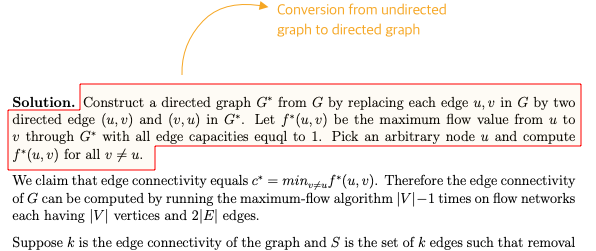
\includegraphics[width=\linewidth]{images/worksheet_5_solution_23.png}
        \end{center}

        \bigskip

        And they all are relevant to the solution.

        \item I feel the solution was being super careful about not mentioning flow network

        \begin{itemize}
            \item Flow network cannot have anti-parallel edges
        \end{itemize}

        \item I noticed that the professor used the word 'claim' when he came up
        with his own algorithm that finds edge connectivity.

        \item \textbf{Maximum Flow:}

        \begin{itemize}
            \item \st{Is a vertex in flow network with the maximum value of flow}
            \item Is equal to the capacity of minimum cut (Corollary 26.5)
        \end{itemize}

        \item \textbf{Edge Connectivity:} Is the minimum number $k$ of edges
        that must be removed to disconnect the graph. That is, the \textbf{number of edges
        in a smallest cut set of G} $^{[2]}$

        \bigskip

        \underline{\textbf{Example:}}

        \bigskip

        \begin{center}
        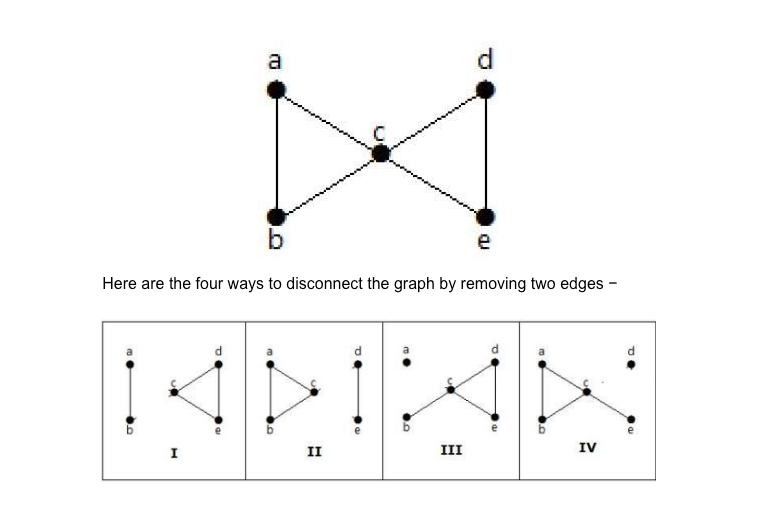
\includegraphics[width=\linewidth]{images/worksheet_5_solution_22.png}
        \end{center}

        \item \textbf{Connected:} A graph is said to be connected if there is a path
        between \ul{every pair of vertex}

        \bigskip

        \underline{\textbf{Example:}}

        \bigskip

        \begin{center}
        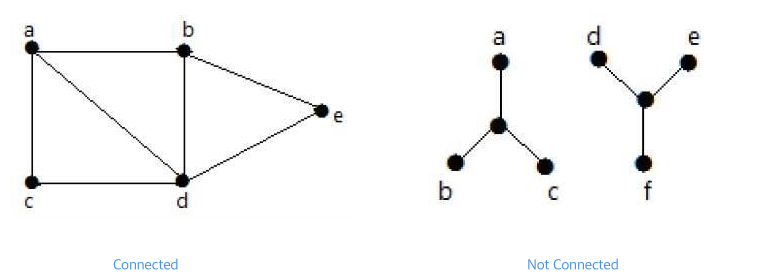
\includegraphics[width=\linewidth]{images/worksheet_5_solution_21.png}
        \end{center}
    \end{itemize}

    \bigskip

    \underline{\textbf{References}}

    \bigskip

    \begin{enumerate}[1)]
        \item National Taiwan University, Voluntary Exercise 3, \href{https://www.csie.ntu.edu.tw/~r95122/alg07spr/alg07spr_hw3sol.pdf}{link}
        \item TutorialsPoint, Graph Theory - Connectivity, \href{https://www.tutorialspoint.com/graph_theory/graph_theory_connectivity.htm}{link}
    \end{enumerate}

    \item


    \bigskip

    \underline{\textbf{Rough Works}}
    \setcounter{equation}{0}
    \bigskip

    Given the flow network $G$ we will produce a flow network $G'$ such that any minimum
    cut in $G'$ is a minimum cut in $G$ with the smallest number of edges (note that the minimum cut)
    with the smallest number of edges might not be unique). Then we execute any max-flow algorithm on
    $G'$ determine any min-cut of $G'$ and return the corresponding cut in $G$.

    \bigskip

    Let $G = (V,E)$ be a flow network in integral capacities $c_e \geq 0$, $e \in E$.
    We define the flow network $G' = (V,E)$ with edge capacities $c'_e \geq 0$, $e \in E$
    and we set $c'_e := \lvert E \rvert \cdot c_e + 1$.

    \bigskip

    \textbf{Claim:} Any min-cut in $G'$ is a min-cut of $G$ with a smallest number of edges.

    \bigskip

\

    \bigskip

    Let $(S,V \setminus S)$ be a min cut in $G'$ and let $F$ be the set of edges
    crossing the cut. Then the capacity of the cut in $G'$ is $\sum\limits_{e \in F} c'_e = \sum\limits_{c \in F} (\lvert E \rvert c_e + 1)
    = \lvert F \rvert + \lvert E \rvert \sum\limits_{c \in F} c_e$ and the capacity of the
    corresponding cut in $G$ is $C_G(S) := \sum\limits_{e \in F} c_e$.

    \bigskip

    We prove the claim by contradiction. At first assume that $(S, V \setminus S)$ is not
    a min-cut in $G$, i.e. there is a cut $(S', V \setminus S')$ in $G$ with capacity smaller than
    $C_G(S)$. Let $F'$ be the edges crossing this cut. Then the cut in $G'$ has capacity

    \bigskip

    \begin{mdframed}
    \underline{\textbf{My Work}}

    \begin{align}
        \sum\limits_{e \in F'} c'_e &= \sum\limits_{e \in F'} (\lvert E \rvert \cdot c_e + 1)\\
        &= \lvert E \rvert \sum\limits_{e \in F'} c_e + \sum\limits_{e \in F'} 1\\
        &= \lvert E \rvert \sum\limits_{e \in F'} c_e + \lvert F' \rvert\\
        &\leq \lvert E \rvert (\sum\limits_{e \in F}c_e - 1) + \lvert F' \rvert & [\text{Since $0 \leq \sum\limits_{e \in F'} c_e < \sum\limits_{e \in F}c_e$}]\\
        &\leq \lvert E \rvert (\sum\limits_{e \in F}c_e - 1) + \lvert E \rvert & [\text{Since $\lvert F \rvert \leq \lvert E \rvert$}]\\
        &= \lvert E \rvert \sum\limits_{e \in F}c_e - \lvert E \rvert + \lvert E \rvert\\
        &= \lvert E \rvert \sum\limits_{e \in F}c_e\\
        &\leq \lvert E \rvert \sum\limits_{e \in F}c_e + \lvert F \rvert\\
        &= \sum\limits_{e \in F}(\lvert E \rvert \cdot c_e + 1)\\
        &= \sum\limits_{e \in F}c'_e
    \end{align}
    \end{mdframed}

    This is a contradction to $(S, V \setminus S)$ being a minimum cut of $G'$.

    \bigskip

    Now, we know that $(S, V \setminus S)$ is a minimum cut of $G$. Now, assume that there
    is a minimum cut $(S', V \setminus S')$ of $G$ that uses fewer edges than the cut $S$.
    Again let $F'$ be the edges crossing this cut. Then we can perform a similar calulation
    as above and we obtain that the cut $S'$ in $G'$ has capacity

    \begin{mdframed}
    \underline{\textbf{My Work}}
    \end{mdframed}

    This is a contradiction to $(S, V \setminus S)$ being a minimum cut of $G'$, which proves the claim.

    \bigskip

    \underline{\textbf{Notes}}

    \bigskip

    \begin{itemize}
        \item \textbf{$A := B$}

        \begin{itemize}
            \item Means $A$ and $B$ are equal by definition (i.e. $A$ is defined as $B$) $^{[3]}$
            \item Feels like the assignment operator $=$ in programming languages

            \bigskip

            \underline{\textbf{Example}}

            \bigskip

            $i := 2$ Means $i$ is defined to have constant value $2$.
        \end{itemize}

        \item \textbf{Cut}

        \begin{itemize}
            \item Is denoted using `a cut $(S,T)$'.
            \item Is a partition of $V$ into $S$ and $T = V - S$ such that $s \in S$ and
            $t \in T$

            \begin{itemize}
                \item \textbf{Partition }means a grouping of its elements into non-empty
                subsets, in such a way that every element is included in exactly one
                subset $^{[2]}$
            \end{itemize}

            \begin{center}
            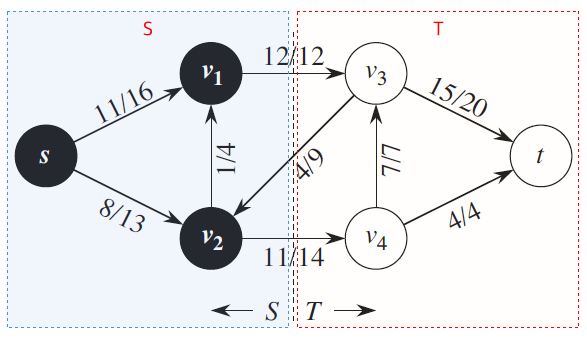
\includegraphics[width=0.5\linewidth]{images/worksheet_5_solution_26.png}
            \end{center}
        \end{itemize}

        \item \textbf{Capacity of a Cut}
        \begin{itemize}
            \item Is used as an \textbf{upper bound} on the flow from source to sink
            \item Arrow in reverse direction is ignored
            \item Is the \underline{maximum flow} that can cross the cut from source to sink
        \end{itemize}

        \bigskip

        \begin{center}
        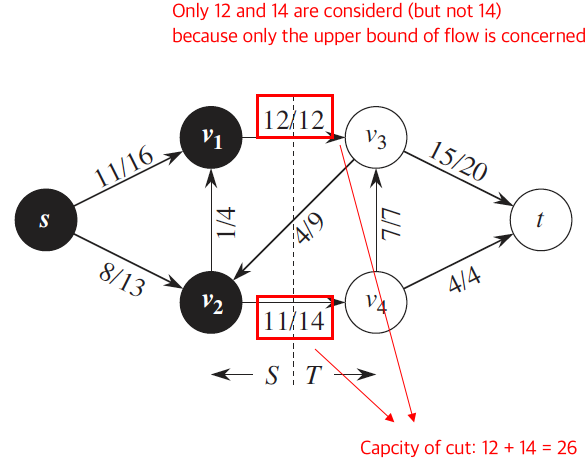
\includegraphics[width=0.5\linewidth]{images/worksheet_5_solution_24.png}
        \end{center}

        \item \textbf{Minimum Cut of a network}

        \begin{itemize}
            \item Is a cut whose capacity is minimum over all cuts of the network
        \end{itemize}


        \begin{center}
        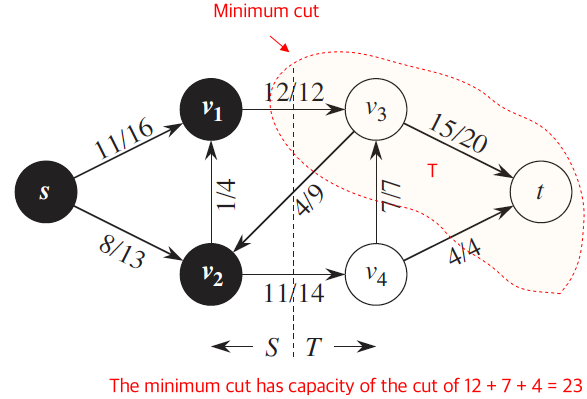
\includegraphics[width=0.5\linewidth]{images/worksheet_5_solution_25.png}
        \end{center}

        \item \textbf{Integral Capacity}

        \begin{itemize}
            \item Means capacity denoted by an integer value
        \end{itemize}
    \end{itemize}

    \bigskip

    \underline{\textbf{References}}

    \bigskip

    \begin{enumerate}[1)]
        \item University of Freiburg, Algorithm Theory, Winter Term 2016/17 Problem Set 5 Sample Solution, \href{http://ac.informatik.uni-freiburg.de/teaching/ws16_17/algo1617/solutions/algo_exercise05_solution.pdf}{link}
        \item Wikipedia, Algorithm Theory, Partition of a set, \href{https://en.wikipedia.org/wiki/Partition_of_a_set#:~:text=In%20mathematics%2C%20a%20partition%20of,partition%20defines%20an%20equivalence%20relation.}{link}
        \item Wolfram Math World, Defined, \href{https://mathworld.wolfram.com/Defined.html}{link}
    \end{enumerate}


\end{enumerate}

\end{document}